\chapter[Solução Proposta]{Solução Proposta}

\section{Arquitetura de Software}
O projeto proposto irá dispor de sistemas de softwares distintos que se comunicam entre si, ao qual irão ser responsáveis pelo controle, recepção e apresentação dos dados aos usuários, oriundos do sensoriamento da transportadora de órgãos.

\subsection{Sistema Interno}

Para o sistema implementado junto ao módulo eletrônico da transportadora será utilizado a linguagem de programação C++, que será responsável pela transmissão e recepção dos dados por meio dos sensores e circuitos. 
Este sistema será integrado junto ao sistema web por meio de arquitetura cliente-servidor ao qual será especificado posteriormente.

\subsubsection{Requisitos funcionais}

\begin{table}[H]
\centering
\begin{tabular}{|
>{\columncolor[HTML]{C0C0C0}}l |l|l|l|}
\hline
\textbf{Identificador} & \multicolumn{3}{l|}{RF001}                                                                                                                                                                      \\ \hline
\textbf{Nome}          & \multicolumn{3}{l|}{Apresentar o nível de pressão da caixa transportadora}                                                                                                                      \\ \hline
\textbf{Módulo}        & \multicolumn{3}{l|}{Sistema interno}                                                                                                                                                            \\ \hline
\textbf{Versão}        & 2                                             & \cellcolor[HTML]{C0C0C0}\textbf{Prioridade}                                             & Essencial                                             \\ \hline
\textbf{Descrição}     & \multicolumn{3}{l|}{\begin{tabular}[c]{@{}l@{}}O sistema deve ser capaz de apresentar o nível de pressão registrado\\ pelo sensor de pressão integrado na caixa transportadora\end{tabular}} \\ \hline
\end{tabular}
\caption{Sistema interno - requisito funcional 001}
\label{RF001}
\end{table}

\begin{table}[H]
\centering
\begin{tabular}{|
>{\columncolor[HTML]{C0C0C0}}l |l|l|l|}
\hline
\textbf{Identificador} & \multicolumn{3}{l|}{RF002}                                                                                                                                                                              \\ \hline
\textbf{Nome}          & \multicolumn{3}{l|}{Apresentar o nível de temperatura da caixa transportadora}                                                                                                                          \\ \hline
\textbf{Módulo}        & \multicolumn{3}{l|}{Sistema interno}                                                                                                                                                                    \\ \hline
\textbf{Versão}        & 2                                                 & \cellcolor[HTML]{C0C0C0}\textbf{Prioridade}                                               & Essencial                                               \\ \hline
\textbf{Descrição}     & \multicolumn{3}{l|}{\begin{tabular}[c]{@{}l@{}}O sistema deve ser capaz de apresentar o nível de temperatura regis-\\trado pelo sensor de temperatura integrado na caixa transportadora\end{tabular}} \\ \hline
\end{tabular}
\caption{Sistema interno - requisito funcional 002}
\label{RF002}
\end{table}

\begin{table}[H]
\centering
\begin{tabular}{|
>{\columncolor[HTML]{C0C0C0}}l |l|l|l|}
\hline
\textbf{Identificador} & \multicolumn{3}{l|}{RF003}                                                                                                                                \\ \hline
\textbf{Nome}          & \multicolumn{3}{l|}{Controlar o nível de temperatura manualmente}                                                                                         \\ \hline
\textbf{Módulo}        & \multicolumn{3}{l|}{Sistema interno}                                                                                                                      \\ \hline
\textbf{Versão}        & 2                                 & \cellcolor[HTML]{C0C0C0}\textbf{Prioridade}                                & Essencial                                \\ \hline
\textbf{Descrição}     & \multicolumn{3}{l|}{\begin{tabular}[c]{@{}l@{}}O usuário é capaz de controlar o nível de temperatura da caixa trans-\\portadora manualmente\end{tabular}} \\ \hline
\end{tabular}
\caption{Sistema interno - requisito funcional 003}
\label{RF003}
\end{table}

\begin{table}[H]
\centering
\begin{tabular}{|
>{\columncolor[HTML]{C0C0C0}}l |l|l|l|}
\hline
\textbf{Identificador} & \multicolumn{3}{l|}{RF004}                                                                                                                            \\ \hline
\textbf{Nome}          & \multicolumn{3}{l|}{Controlar o nível de pressão manualmente}                                                                                         \\ \hline
\textbf{Módulo}        & \multicolumn{3}{l|}{Sistema interno}                                                                                                                  \\ \hline
\textbf{Versão}        & 2                                & \cellcolor[HTML]{C0C0C0}\textbf{Prioridade}                               & Essencial                              \\ \hline
\textbf{Descrição}     & \multicolumn{3}{l|}{\begin{tabular}[c]{@{}l@{}}O usuário é capaz de controlar o nível de pressão da caixa  trans-\\portadora manualmente\end{tabular}} \\ \hline
\end{tabular}
\caption{Sistema interno - requisito funcional 004}
\label{RF004}
\end{table}

\begin{table}[H]
\centering
\begin{tabular}{|
>{\columncolor[HTML]{C0C0C0}}l |l|l|l|}
\hline
\textbf{Identificador} & \multicolumn{3}{l|}{RF005}                                                                                                                                                                                                   \\ \hline
\textbf{Nome}          & \multicolumn{3}{l|}{Controlar o nível da temperatura automaticamente}                                                                                                                                                        \\ \hline
\textbf{Módulo}        & \multicolumn{3}{l|}{Sistema interno}                                                                                                                                                                                         \\ \hline
\textbf{Versão}        & 2                                                        & \cellcolor[HTML]{C0C0C0}\textbf{Prioridade}                                                      & Essencial                                                      \\ \hline
\textbf{Descrição}     & \multicolumn{3}{l|}{\begin{tabular}[c]{@{}l@{}}O sistema deve ser capaz de sensoriar e controlar a o nível de\\ temperatura da caixa transportadora automaticamente de acordo\\ com o órgão a ser transportado\end{tabular}} \\ \hline
\end{tabular}
\caption{Sistema interno - requisito funcional 005}
\label{RF005}
\end{table}

\begin{table}[H]
\centering
\begin{tabular}{|
>{\columncolor[HTML]{C0C0C0}}l |l|l|l|}
\hline
\textbf{Identificador} & \multicolumn{3}{l|}{RF006}                                                                                                                                                                                               \\ \hline
\textbf{Nome}          & \multicolumn{3}{l|}{Controlar o nível da pressão automaticamente}                                                                                                                                                        \\ \hline
\textbf{Módulo}        & \multicolumn{3}{l|}{Sistema interno}                                                                                                                                                                                     \\ \hline
\textbf{Versão}        & 2                                                      & \cellcolor[HTML]{C0C0C0}\textbf{Prioridade}                                                     & Essencial                                                     \\ \hline
\textbf{Descrição}     & \multicolumn{3}{l|}{\begin{tabular}[c]{@{}l@{}}O sistema deve ser capaz de sensoriar e controlar a o nível de pres-\\são da caixa transportadora automaticamente de acordo\\ com o órgão a ser transportado\end{tabular}} \\ \hline
\end{tabular}
\caption{Sistema interno - requisito funcional 006}
\label{RF006}
\end{table}

\begin{table}[H]
\centering
\begin{tabular}{|
>{\columncolor[HTML]{C0C0C0}}l |l|l|l|}
\hline
\textbf{Identificador} & \multicolumn{3}{l|}{RF007}                                                                                                                                                                                                                                           \\ \hline
\textbf{Nome}          & \multicolumn{3}{l|}{Selecionar parâmetros pré-definidos de acordo com o órgão}                                                                                                                                                                                       \\ \hline
\textbf{Módulo}        & \multicolumn{3}{l|}{Sistema interno}                                                                                                                                                                                                                                 \\ \hline
\textbf{Versão}        & 1                                                                     & \cellcolor[HTML]{C0C0C0}\textbf{Prioridade}                                                                    & Desejável                                                                   \\ \hline
\textbf{Descrição}     & \multicolumn{3}{l|}{\begin{tabular}[c]{@{}l@{}}Quando o usuário escolher o tipo de órgão a ser transportado, o sis-\\tema deve ser capaz de selecionar automaticamente\\ parâmetros de pressão e temperatura pré-definidos para aquele\\ tipo de órgão.\end{tabular}} \\ \hline
\end{tabular}
\caption{Sistema interno - requisito funcional 007}
\label{RF007}
\end{table}

\subsection{Sistema Web}

Para a construção da aplicação proposta foi definido a implementação de um sistema web no qual ficarão dispostas as informações do sensoriamento da transportadora, além de informações de localização pelo GPS integrado. Este sistema terá como servidor a Raspberry Pi e os usuários poderão se conectar e visualizar o transporte do órgão.

Dessa forma, a implementação deste sistema utilizará das seguintes tecnologias:
\begin{itemize}
	\item Linguagem de Programação Python - linguagem de programação de alto nível, multiparadigma, interpretada e de tipagem dinâmica e forte;
    \item  Django Framework - framework para desenvolvimento web, escrito em Python, open source, que utiliza o padrão model-template-view. (MTV), utiliza por padrão banco de dados Sqlite3.
\end{itemize}

\subsubsection{Requisitos funcionais}

\begin{table}[H]
\centering
\begin{tabular}{|
>{\columncolor[HTML]{C0C0C0}}l |l|l|l|}
\hline
\textbf{Identificador} & \multicolumn{3}{l|}{RF008}                                                                                                                                                                               \\ \hline
\textbf{Nome}          & \multicolumn{3}{l|}{Apresentar o nível de pressão da caixa transportadora}                                                                                                                               \\ \hline
\textbf{Módulo}        & \multicolumn{3}{l|}{Sistema Web}                                                                                                                                                                         \\ \hline
\textbf{Versão}        & 2                                                & \cellcolor[HTML]{C0C0C0}\textbf{Prioridade}                                                & Essencial                                                \\ \hline
\textbf{Descrição}     & \multicolumn{3}{l|}{\begin{tabular}[c]{@{}l@{}}O web app deve ser capaz de apresentar ao usuário a informação\\ do nível de pressão advindo do sensor de pressão da caixa\\ transportadora\end{tabular}} \\ \hline
\end{tabular}
\caption{Sistema Web - requisito funcional 008}
\label{RF008}
\end{table}

\begin{table}[H]
\centering
\begin{tabular}{|
>{\columncolor[HTML]{C0C0C0}}l |l|l|l|}
\hline
\textbf{Identificador} & \multicolumn{3}{l|}{RF009}                                                                                                                                                                                       \\ \hline
\textbf{Nome}          & \multicolumn{3}{l|}{Apresentar o nível de temperatura da caixa transportadora}                                                                                                                                   \\ \hline
\textbf{Módulo}        & \multicolumn{3}{l|}{Sistema Web}                                                                                                                                                                                 \\ \hline
\textbf{Versão}        & 2                                                    & \cellcolor[HTML]{C0C0C0}\textbf{Prioridade}                                                  & Essencial                                                  \\ \hline
\textbf{Descrição}     & \multicolumn{3}{l|}{\begin{tabular}[c]{@{}l@{}}O web app deve ser capaz de apresentar ao usuário a informação\\ do nível de temperatura advindo do sensor de temperatura da\\ caixa transportadora\end{tabular}} \\ \hline
\end{tabular}
\caption{Sistema Web - requisito funcional 009}
\label{RF009}
\end{table}

\begin{table}[H]
\centering
\begin{tabular}{|
>{\columncolor[HTML]{C0C0C0}}l |l|l|l|}
\hline
\textbf{Identificador} & \multicolumn{3}{l|}{RF010}                                                                                                                                                         \\ \hline
\textbf{Nome}          & \multicolumn{3}{l|}{Apresentar a localização em tempo real da caixa transportadora}                                                                                                \\ \hline
\textbf{Módulo}        & \multicolumn{3}{l|}{Sistema Web}                                                                                                                                                   \\ \hline
\textbf{Versão}        & 2                                         & \cellcolor[HTML]{C0C0C0}\textbf{Prioridade}                                         & Essencial                                        \\ \hline
\textbf{Descrição}     & \multicolumn{3}{l|}{\begin{tabular}[c]{@{}l@{}}O web app deve ser capaz de apresentar a localização em tempo\\ real advindo do GPS integrado na caixa transportadora\end{tabular}} \\ \hline
\end{tabular}
\caption{Sistema Web - requisito funcional 010}
\label{RF010}
\end{table}

\begin{table}[H]
\centering
\begin{tabular}{|
>{\columncolor[HTML]{C0C0C0}}l |l|l|l|}
\hline
\textbf{Identificador} & \multicolumn{3}{l|}{RF011}                                                            \\ \hline
\textbf{Nome}          & \multicolumn{3}{l|}{Cadastrar médicos}                                                \\ \hline
\textbf{Módulo}        & \multicolumn{3}{l|}{Sistema Web}                                                      \\ \hline
\textbf{Versão}        & 2          & \cellcolor[HTML]{C0C0C0}\textbf{Prioridade}          & Essencial         \\ \hline
\textbf{Descrição}     & \multicolumn{3}{l|}{\begin{tabular}[c]{@{}l@{}}O web app deve permitir o cadastro de médicos certificados com\\
CRM\end{tabular}} \\ \hline
\end{tabular}
\caption{Sistema Web - requisito funcional 011}
\label{RF011}
\end{table}

\begin{table}[H]
\centering
\begin{tabular}{|
>{\columncolor[HTML]{C0C0C0}}l |l|l|l|}
\hline
\textbf{Identificador} & \multicolumn{3}{l|}{RF012}                                                                                                                         \\ \hline
\textbf{Nome}          & \multicolumn{3}{l|}{Possuir nível de acesso admin}                                                                                                 \\ \hline
\textbf{Módulo}        & \multicolumn{3}{l|}{Sistema Web}                                                                                                                   \\ \hline
\textbf{Versão}        & 2                              & \cellcolor[HTML]{C0C0C0}\textbf{Prioridade}                              & Essencial                              \\ \hline
\textbf{Descrição}     & \multicolumn{3}{l|}{\begin{tabular}[c]{@{}l@{}}O web app deve possuir um nível de acesso de administrador com\\ privilégios próprios\end{tabular}} \\ \hline
\end{tabular}
\caption{Sistema Web - requisito funcional 012}
\label{RF012}
\end{table}

\begin{table}[H]
\centering
\begin{tabular}{|
>{\columncolor[HTML]{C0C0C0}}l |l|l|l|}
\hline
\textbf{Identificador} & \multicolumn{3}{l|}{RF013}                                                                                                                                         \\ \hline
\textbf{Nome}          & \multicolumn{3}{l|}{Possuir nível de acesso médico}                                                                                                                \\ \hline
\textbf{Módulo}        & \multicolumn{3}{l|}{Sistema Web}                                                                                                                                   \\ \hline
\textbf{Versão}        & 2                                    & \cellcolor[HTML]{C0C0C0}\textbf{Prioridade}                                   & Essencial                                   \\ \hline
\textbf{Descrição}     & \multicolumn{3}{l|}{\begin{tabular}[c]{@{}l@{}}O web app deverá possuir um nível de acesso para médicos, o qual\\ é inferior o nível de acesso admin\end{tabular}} \\ \hline
\end{tabular}
\caption{Sistema Web - requisito funcional 013}
\label{RF013}
\end{table}

\begin{table}[H]
\centering
\begin{tabular}{|
>{\columncolor[HTML]{C0C0C0}}l |l|l|l|}
\hline
\textbf{Identificador} & \multicolumn{3}{l|}{RF014}                                                                                                                                                \\ \hline
\textbf{Nome}          & \multicolumn{3}{l|}{Apresentar informações do órgão a ser transportado}                                                                                                   \\ \hline
\textbf{Módulo}        & \multicolumn{3}{l|}{Sistema Web}                                                                                                                                          \\ \hline
\textbf{Versão}        & 1                                      & \cellcolor[HTML]{C0C0C0}\textbf{Prioridade}                                      & Desejável                                     \\ \hline
\textbf{Descrição}     & \multicolumn{3}{l|}{\begin{tabular}[c]{@{}l@{}}O web app deve ser capaz de apresentar algumas informações do ór-\\gão que está sendo transportado no momento\end{tabular}} \\ \hline
\end{tabular}
\caption{Sistema Web - requisito funcional 014}
\label{RF014}
\end{table}

\begin{table}[H]
\centering
\begin{tabular}{|
>{\columncolor[HTML]{C0C0C0}}l |l|l|l|}
\hline
\textbf{Identificador} & \multicolumn{3}{l|}{RF015}                                                                                                                                                                                                                                                                                   \\ \hline
\textbf{Nome}          & \multicolumn{3}{l|}{Gerar relatório do processo de transporte do órgão}                                                                                                                                                                                                                                      \\ \hline
\textbf{Módulo}        & \multicolumn{3}{l|}{Sistema Web}                                                                                                                                                                                                                                                                             \\ \hline
\textbf{Versão}        & 1                                                                                  & \cellcolor[HTML]{C0C0C0}\textbf{Prioridade}                                                                                 & Desejável                                                                                 \\ \hline
\textbf{Descrição}     & \multicolumn{3}{l|}{\begin{tabular}[c]{@{}l@{}}O web app deve ser capaz de gerar um relatório final com registros\\ do processo de transporte de algum órgão específico.\\ Como por exemplo: a variação de temperatura e pressão, o\\ registro do deslocamento (origem, destino e percurso)...\end{tabular}} \\ \hline
\end{tabular}
\caption{Sistema Web - requisito funcional 015}
\label{RF015}
\end{table}

\section{Sistema de Refrigeração}
A refrigeração da câmara tem como base o uso da pastilhas termo elétricas, denominadas de módulos Peltier que são pequenas unidades que utilizam tecnologia de matéria condensada para operarem como bombas de calor. Esta pastilha é feita de material semicondutor e é capaz de causar um diferença de temperatura nas suas faces quando submetida à uma tensão.

\subsection{Estrutura do conjunto de refrigeração}
Pelas especificações do projeto em ser um ambiente de refrigeração para o transporte de órgãos para transplante, a face de menor temperatura da célula peltier deve estar em contato com o ar de dentro da câmara para que assim ocorra o seu resfriamento. Já o lado de maior temperatura da célula peltier deve estar em contato com o ar circundante no ambiente externo, tornando assim a troca de calor entre as duas regiões mais eficaz.

Em vista disso, serão utilizados dois dissipadores de calor, que estarão em contato direto com uma pasta térmica, e esta irá em contato com o módulo peltier. Logo acima das colmeias de cada dissipador haverá um cooler, que tem como principal objetivo melhorar a circulação de ar pelos dissipadores, consequentemente tornar a troca de calor do sistema ainda mais eficiente.

Na figura abaixo é apresentada uma visão explodida da solução de refrigeração:

\begin{figure}[H]
\begin{center}
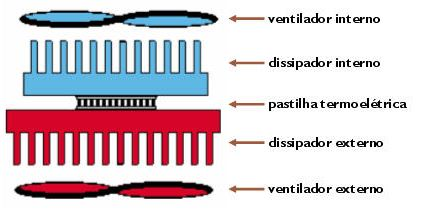
\includegraphics[scale = 1]{figuras/Sistema_Ref.JPG}
\caption{Visão explodida do sistema de refrigeração}
\end{center}
\end{figure}

O desempenho dos módulos peltier é diretamente proporcional às grandezas que o controlam. Devido a esta característica, para um projeto o fabricante disponibiliza um conjunto de curvas que irão permitir ao projetista determinar os limites seguros de operação do sistema de refrigeração. Algumas combinações dessas grandezas podem tornar o sistema que possui um comportamento ótimo para um desempenho inadmissível. 

\begin{table}[H]
\begin{center}
\caption{Dados de Desempenho da Célula Peltier. FONTE: Folha de Dados TEC-12706 – HB Eletronic Components.}
\begin{tabular}{|c|c|c|}
\hline
\textbf{Temperatura do lado quente (ºC)} & 25 & 50  \\
\hline
\textbf{$Q_{MAX}$ (W)} & 50 & 57 \\
\hline
\textbf{$\Delta T_{MAX}$ (ºC)}& 66 & 75 \\
\hline
\textbf{$I_{MAX}$ (A)} & 6,4 & 6,4 \\
\hline
\textbf{$V_{MAX}$ (V)} & 14,14 & 16,4 \\
\hline 
\textbf{Resistência do Módulo ($\Omega$)} & 1,98 & 2,3\\
\hline
\end{tabular}

\end{center}
\end{table}
\subsection{Dimensionamento do sistema de refrigeração Peltier}
O dimensionamento do sistema de refrigeração por Peltier irá ser desenvolvido de modo sistemático, tendo como referência a definição de uma carga térmica e a diferença de temperatura quente/frio (DT) [1]. Cabe alertar que serão determinados pontos ótimos de operação e uma estimativa de desempenho para o sistema uma vez que o sistema tem um comportamento não-linear. 

\subsubsection{Determinação das temperaturas de trabalho}
Serão definidas nesta etapa as temperaturas de trabalho, afim de:
\begin{itemize}
	\item Fazer a escolha do módulo peltier;
    \item Escolher o dissipador de calor para o módulo;
    \item Calcular as cargas térmicas do projeto. 
\end{itemize}
Portanto, as temperaturas de trabalho estão assim estabelecidas:
\begin{table}[H]
\caption{ Temperaturas de trabalho do módulo Peltier}
\begin{tabular}{c|c|c}
     &  \textbf{Temperatura (ºC)} & \textbf{Observação}\\
   \hline
   $T_{ambiente}$ & 35 & Temperatura ambiente em que o dispositivo vai trabalhar \\
   $T_Q$ & 40  & 
Temperatura de trabalho da face quente - dissipador \\
$T_F$ & 0 & Temperatura de trabalho da face fria \\
$\Delta T$ & 40 & 
Os limites do módulo estão ligados a esta variável\\
\hline
\end{tabular}
\end{table}

\subsubsection{Determinação da Carga Térmica}
Existem dois tipos de carga térmica que o sistema de refrigeração vai estar submetido, a carga térmica ativa que é a energia térmica dissipada pelo dispositivo que estará sendo refrigerado, e a carga térmica passiva, a qual é a energia térmica proveniente de radiação, convecção ou condução, ou ainda a combinação dos dois. 

\begin{equation}
Q_{Térmica} = Q_{Radiação}+Q_{Condução}+Q_{Convecção}+Q_{Ativa}
\end{equation}
Descobrir e minimizar as cargas térmicas atuantes no sistema nos permitirá alcançar o nível de refrigeração requisitado e a potência necessária para alcançá-la. A seguir serão estimadas as cargas ativa e passiva do sistema.
\begin{itemize}
\item Carga Térmica Ativa

Esta  fonte é relacionada à presença de dispositivos, no caso em questão à presença do cooler, na região a ser refrigerada e esta carga é representada pela potência dissipada por efeito Joule:
\begin{equation}
Q_{Ativa} = V \times I
\end{equation}
Onde:

$Q_{Ativa}$ --- Potência ativa, em Watts;

V --- Tensão de alimentação do dispositivo (12 V);


I --- Corrente no dispositivo (0,15 A).

O que leva a concluir que a carga térmica ativa é de aproximadamente 1,8 Watts.

\item Carga Térmica Passiva

Para este projeto o cálculo da carga térmica de radiação será desprezado, pois o sistema não trabalha com altas temperaturas à vácuo.

Para o cálculo da carga térmica passiva será utilizada a combinação dos fenômenos de condução e convecção:
\begin{equation}
	Q_{Passivo}= \frac{A \times \Delta T}{\frac{x}{k} + \frac{1}{h}}
\end{equation}
Para o cálculo da área externa foram utilizadas as dimensões externas da câmara de $6\times(300 \times 300)\times 10^{-6}=0,54mm^2$. 

Considerando duas possibilidades de isolantes térmicos que podem ser utilizados no projeto (Poliestireno Expandido e Espuma de Poliuretano), obtêm-se:

Poliestireno expandido (EPS) --- Isopor: 0,045 a 0,034 $\left[\frac{W}{m.K}\right]$ e espessura x=0,02m.

Espuma de poliuretano: 0,023$\left[\frac{W}{m.K}\right]$ e espessura 0,03 m.

Foi utilizado o coeficiente de transferência de calor por convecção do ar por convecção forçada: $h = 250 \left[\frac{@}{M^2.ºC}\right] $

Obtendo assim, duas cargas térmicas passivas:

$Q_{Passiva, Isopor}$ = 24,73 W

$Q_{Passiva, Espuma} $ = 26,51 W

Como as duas cargas são comparativamente próximas, para fins práticos de cálculo será escolhida a maior dentre elas.

Logo, $Q_{Térmica}$ = 28,31 W.

\end{itemize}

\subsubsection{Determinação de Estágios para o Módulo}
Com base nas definições de temperaturas realizadas anteriormente, pode-se determinar portanto o número de estágios do módulo necessários para que o $\Delta T$ seja atingido com segurança.

Com base nas definições de temperaturas realizadas anteriormente, pode-se determinar portanto o número de estágios do módulo necessários para que o T seja atingido com segurança.

\begin{table}[H]
\begin{center}
\caption{Diferença máxima de temperatura para módulos simples e de dois e três estágios}
\begin{tabular}{c||c}
\textbf{Número de Estágios} & \textbf{$\Delta T Max$} 1 atm de $N_2$\\
\hline \hline
1 & 64\\
2 & 84 \\
3 & 95\\
\hline \hline
\end{tabular}
\end{center}
\end{table}

\subsubsection{ Escolha da Célula de Peltier}
Com base no método dimensionamento por carga térmica, é necessária uma célula de Peltier de 28,31  W para climatizar um compartimento de transporte.

Para esse projeto então, será utilizada para fazer a função de climatização do compartimento de transporte de órgãos uma célula de Peltier, cujo modelo adotado foi o TEC1-12706, por ser de fácil acesso no mercado e suprir as necessidades do projeto, conforme os cálculos de dimensionamento por carga térmica realizados. Este modelo possui comprimento e largura de 4cm e altura de 3,2mm. A corrente elétrica máxima que esta célula de peltier pode suportar é de 6 Ampères, a tensão máxima é de 15,4V e a potência máxima é de 63W. 

\subsubsection{Controle do Cooler}

Para controlar a velocidade do cooler será utilizado um controle PWM de forma em que o tempo em que a onda fica em nível lógico alto em relação a todo o período da onda determina a porcentagem de potência entregue ao sistema, e forma a ajustar o consumo de energia para evitar que o consumo de energia seja muito alto desnecessariamente.

\subsubsection{Controle da Célula Peltier}

Da mesma forma que  o cooler o consumo do peltier será estimado pelo controle via PMW, como no caso do peltier se faz necessário o uso de uma tensão de 12V será usado um controle de interrupção simples utilizando transistor MOSFET para atuar como chave que será controlada pelo próprio PWM.

\subsection{Requisitos do Sistema}

Com vistas à concepção e validação da solução, foram definidos os requisitos relativos ao subsistema de alimentação e refrigeração do produto:

\subsubsection{Requisitos Funcionais}
O sistema de refrigeração deve ser capaz de:
\begin{itemize}
\item Refrigerar uma câmara hermeticamente;
\item sistema deve ser capaz de estabilizar a temperatura interna da câmara de forma que o órgão fique com temperatura entre 2ºC e 4ºC;
\item O sistema deve ser capaz de manter a temperatura da câmara uniforme.

\end{itemize}
\subsubsection{Requisitos Não-Funcionais}
O sistema de refrigeração deve ser capaz de:
\begin{itemize}
\item Utilizar dissipadores de calor e células de peltier;
Ser eficiente energeticamente, consumindo o mínimo de consumo possível através de um controle de potência;
\item A câmara a ser refrigerada deve ter um volume máximo de 4 litros;
\item O sistema deve ser capaz de refrigerar o sistema de forma satisfatória durante um período máximo de 48 horas.
\end{itemize}

\section{Sistema de Alimentação}
As fontes de energia que serão utilizadas para alimentar o produto, incluindo o sistema de refrigeração e os componentes elétricos e eletrônicos, são a rede elétrica comum brasileira e um banco de baterias. O banco de baterias será dimensionada afim de manter os subsistemas em perfeita operação durante o período solicitado de 48 horas.

\subsection{Diagrama do Sistema}
A Figura a seguir apresenta o diagrama elétrico simplificado do produto. Ele representa o circuito de alimentação utilizado, desde a fonte de energia --- rede elétrica padrão --- até o uso final em seus componentes elétricos e eletrônicos.  É importante ressaltar que este diagrama será refinado ao longo dos pontos de controle, pois o  sistema pode ser retificado para melhor atender às condições de contorno que forem encontradas durante a execução do projeto.

\begin{figure}[H]
\begin{center}
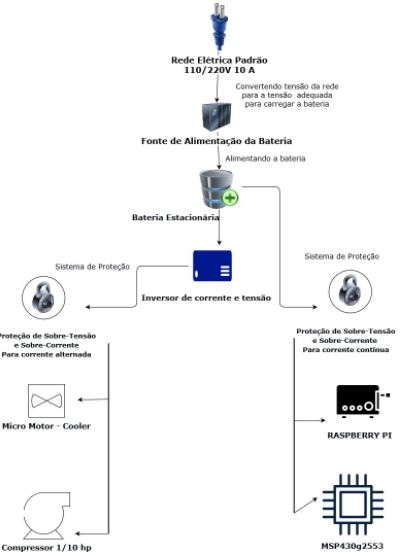
\includegraphics[scale = 1.2]{figuras/Diagrama_Simp.JPG}
\caption{ Diagrama Elétrico Preliminar}
\end{center}
\end{figure}

O sistema foi dimensionado com um fator de segurança elevado, pois a proposta de projeto é de um sistema de acondicionamento de órgãos para transplante. Sendo assim, o nível de confiabilidade do produto deve ser extremamente alto, para isso todo o sistema de alimentação foi dimensionado relacionando o sistema ao tempo de operação necessário ao transporte e diretamente ao consumo de energia advinda da bateria.

\subsection{Baterias}
Baterias têm a finalidade de armazenar energia e liberá-la em determinada periodicidade, e de forma controlada. Sua escolha deve ser adequada às necessidades de consumo energético do projeto, e considera os dados de corrente elétrica e tensão. Para a seleção da bateria adequada deve-se estudar se ela é capaz de armazenar a energia total demandada às necessidades do projeto, e se ela consegue entregar toda a energia necessária ao funcionamento do equipamento.

Dentre as opções de bateria disponíveis no mercado, optou-se pela bateria estacionária. Sua vida útil é de aproximadamente 5 anos, devido à sua composição com materiais internos mais sobres se comparada às baterias automotivas, por exemplo. Podem, também, suportar descargas de até 80\% de sua capacidade, sem prejudicar sua vida útil, e resistem a ciclos de carga ou descarga mais profundos. Tais características proporcionam maior confiabilidade ao funcionamento do projeto pelo uso da bateria estacionaria.

O dimensionamento da bateria requer inicialmente a relação de potência demandada para suprir as necessidades dos componentes elétricos do projeto, como mostra a tabela a seguir:

\begin{table}[H]
\caption{Consumo energético dos componentes}
\begin{tabular}{|p{4 cm} |c |c |c |}
 \hline
   \textbf{COMPONENTE} &\textbf{ALIMENTAÇÃO (V)}  &\textbf{CORRENTE (A)} & \textbf{POTÊNCIA (W)} \\
   \hline
  \textbf{MSP430g2553} &5 & 330$\mu$& 1,65 mW \\
   \hline
   \textbf{RASPBERRY PI}&5 &2,5 & 12,5 \\
   \hline
  \textbf{PROTETOR } &12 &26,5m &318m \\
   \hline
  \textbf{CONTROLADOR PELTIER} &12 & 2,4& 28,33 \\
   \hline
  \textbf{CONTROLADOR COOLER} &12 &260,9m &3,6  \\
   \hline
  \textbf{MÓDULO PWM} &12 &100m & 1,2 \\
   \hline
\end{tabular}
\end{table}

Conhecer a capacidade da bateria e o tempo de uso do equipamento também são necessários ao dimensionamento.

O dimensionamento da bateria foi feito usando as seguintes equações:
\begin{equation}
Consumo = (P) \times (T)
\end{equation}
Onde: 

 P --- Potência em KW;
 T --- Tempo em horas.

%%%%%%%%%%%%%% REVER ESSA PARTE
De acordo com o estimado de carga para o projeto até o momento, teremos a potência em watt de aproximadamente 58,44W, autonomia de 48h e uma bateria com 12V. 

De acordo com o estimado de carga para o projeto até o momento, encontra-se a potência em Watt de 58,44w, o tempo de 48h e uma bateria com 12V  Obtendo valores de, respectivamente: 2,805 $KWh$ e 233,76 $Ah$. Dessa forma, considerando que a tabela acima considera sempre a pior das hipóteses, o valor prático poderá ser redimensionado, de forma que os testes serão iniciados a partir da ligação de 3 baterias de 70 Ah em paralelo.

\subsection{Requisitos}
Com vistas à concepção e validação da solução, foram definidos os requisitos relativos ao subsistema de alimentação e refrigeração do produto:

\subsubsection{Requisitos Funcionais}
O sistema de alimentação deve ser capaz de:
\begin{itemize}
\item Armazenar energia elétrica;
 \item Fornecer energia para os componentes elétricos e eletrônicos de controle e monitoramento do produto;
 \item Fornecer energia para o sistema de refrigeração.
 \end{itemize}
\subsubsection{Requisitos Não Funcionais}
O sistema de alimentação deve ser capaz de:
\begin{itemize}
\item Prover a energia necessária para o bom funcionamento do produto durante um período máximo de 48 horas, com armazenamento de energia em baterias;
\item O sistema deve ser capaz de controlar a potência que será entregue as placas de peltier;
 \item Possuir eficiência energética aceitável, através de um controle de potência no sistema de refrigeração, escolha de componentes eletrônicos de baixa potência e sistemas de standby em determinados componentes não críticos do produto;
 \item Ser estável energeticamente, evitando picos de potência com componentes e segurança de circuitos.
 \end{itemize}

\section{Estrutura}

\subsection{Arquitetura da estrutura}
A estrutura da transportadora de órgãos será feita considerando como principais fatores a  mobilidade e a capacidade de comportar todos os sistemas cumprindo os requisitos de projeto. Além disso, desejou-se aproximar o centro de massa o mais no centro possível da estrutura geral para gerar estabilidade.

Os esquemáticos a seguir mostram de forma simplificada as dimensões, composição e disposição dos elementos estruturais.

\begin{figure}[H]
\centering
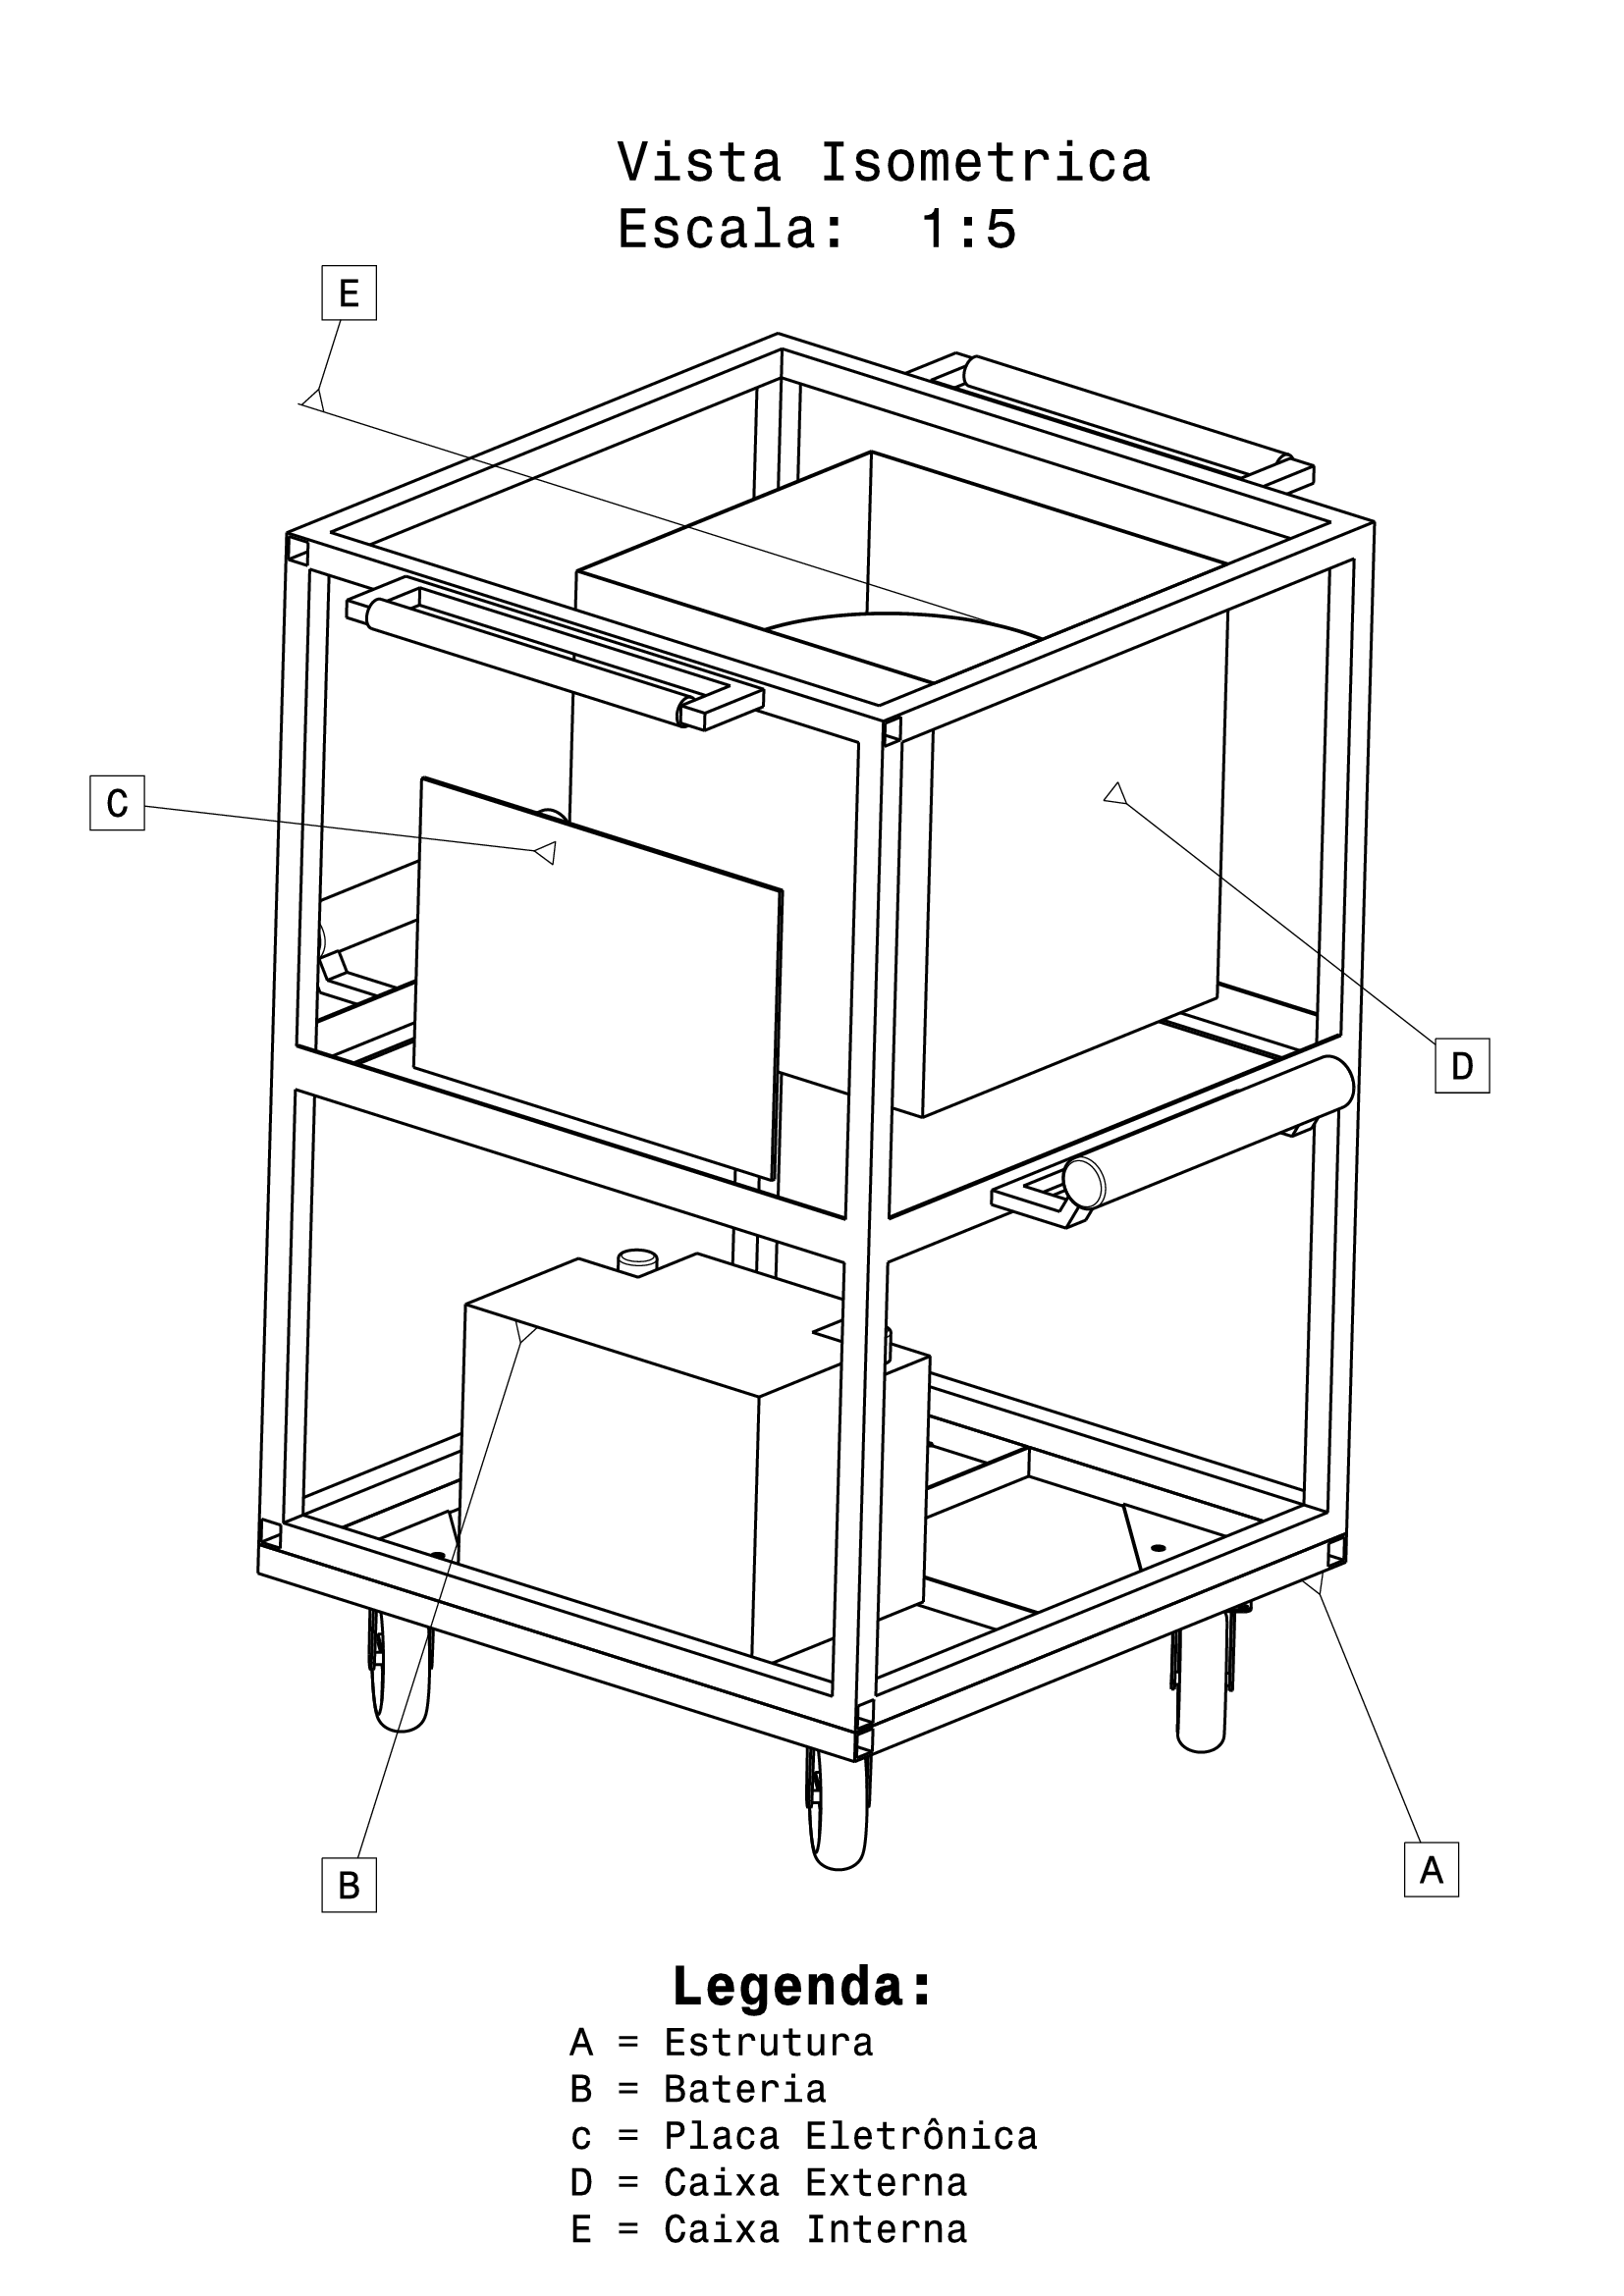
\includegraphics[scale=0.15]{figuras/estrutura.png}
\caption{Estrutura básica da transportadora de órgãos}
\end{figure}

\begin{figure}[H]
\centering
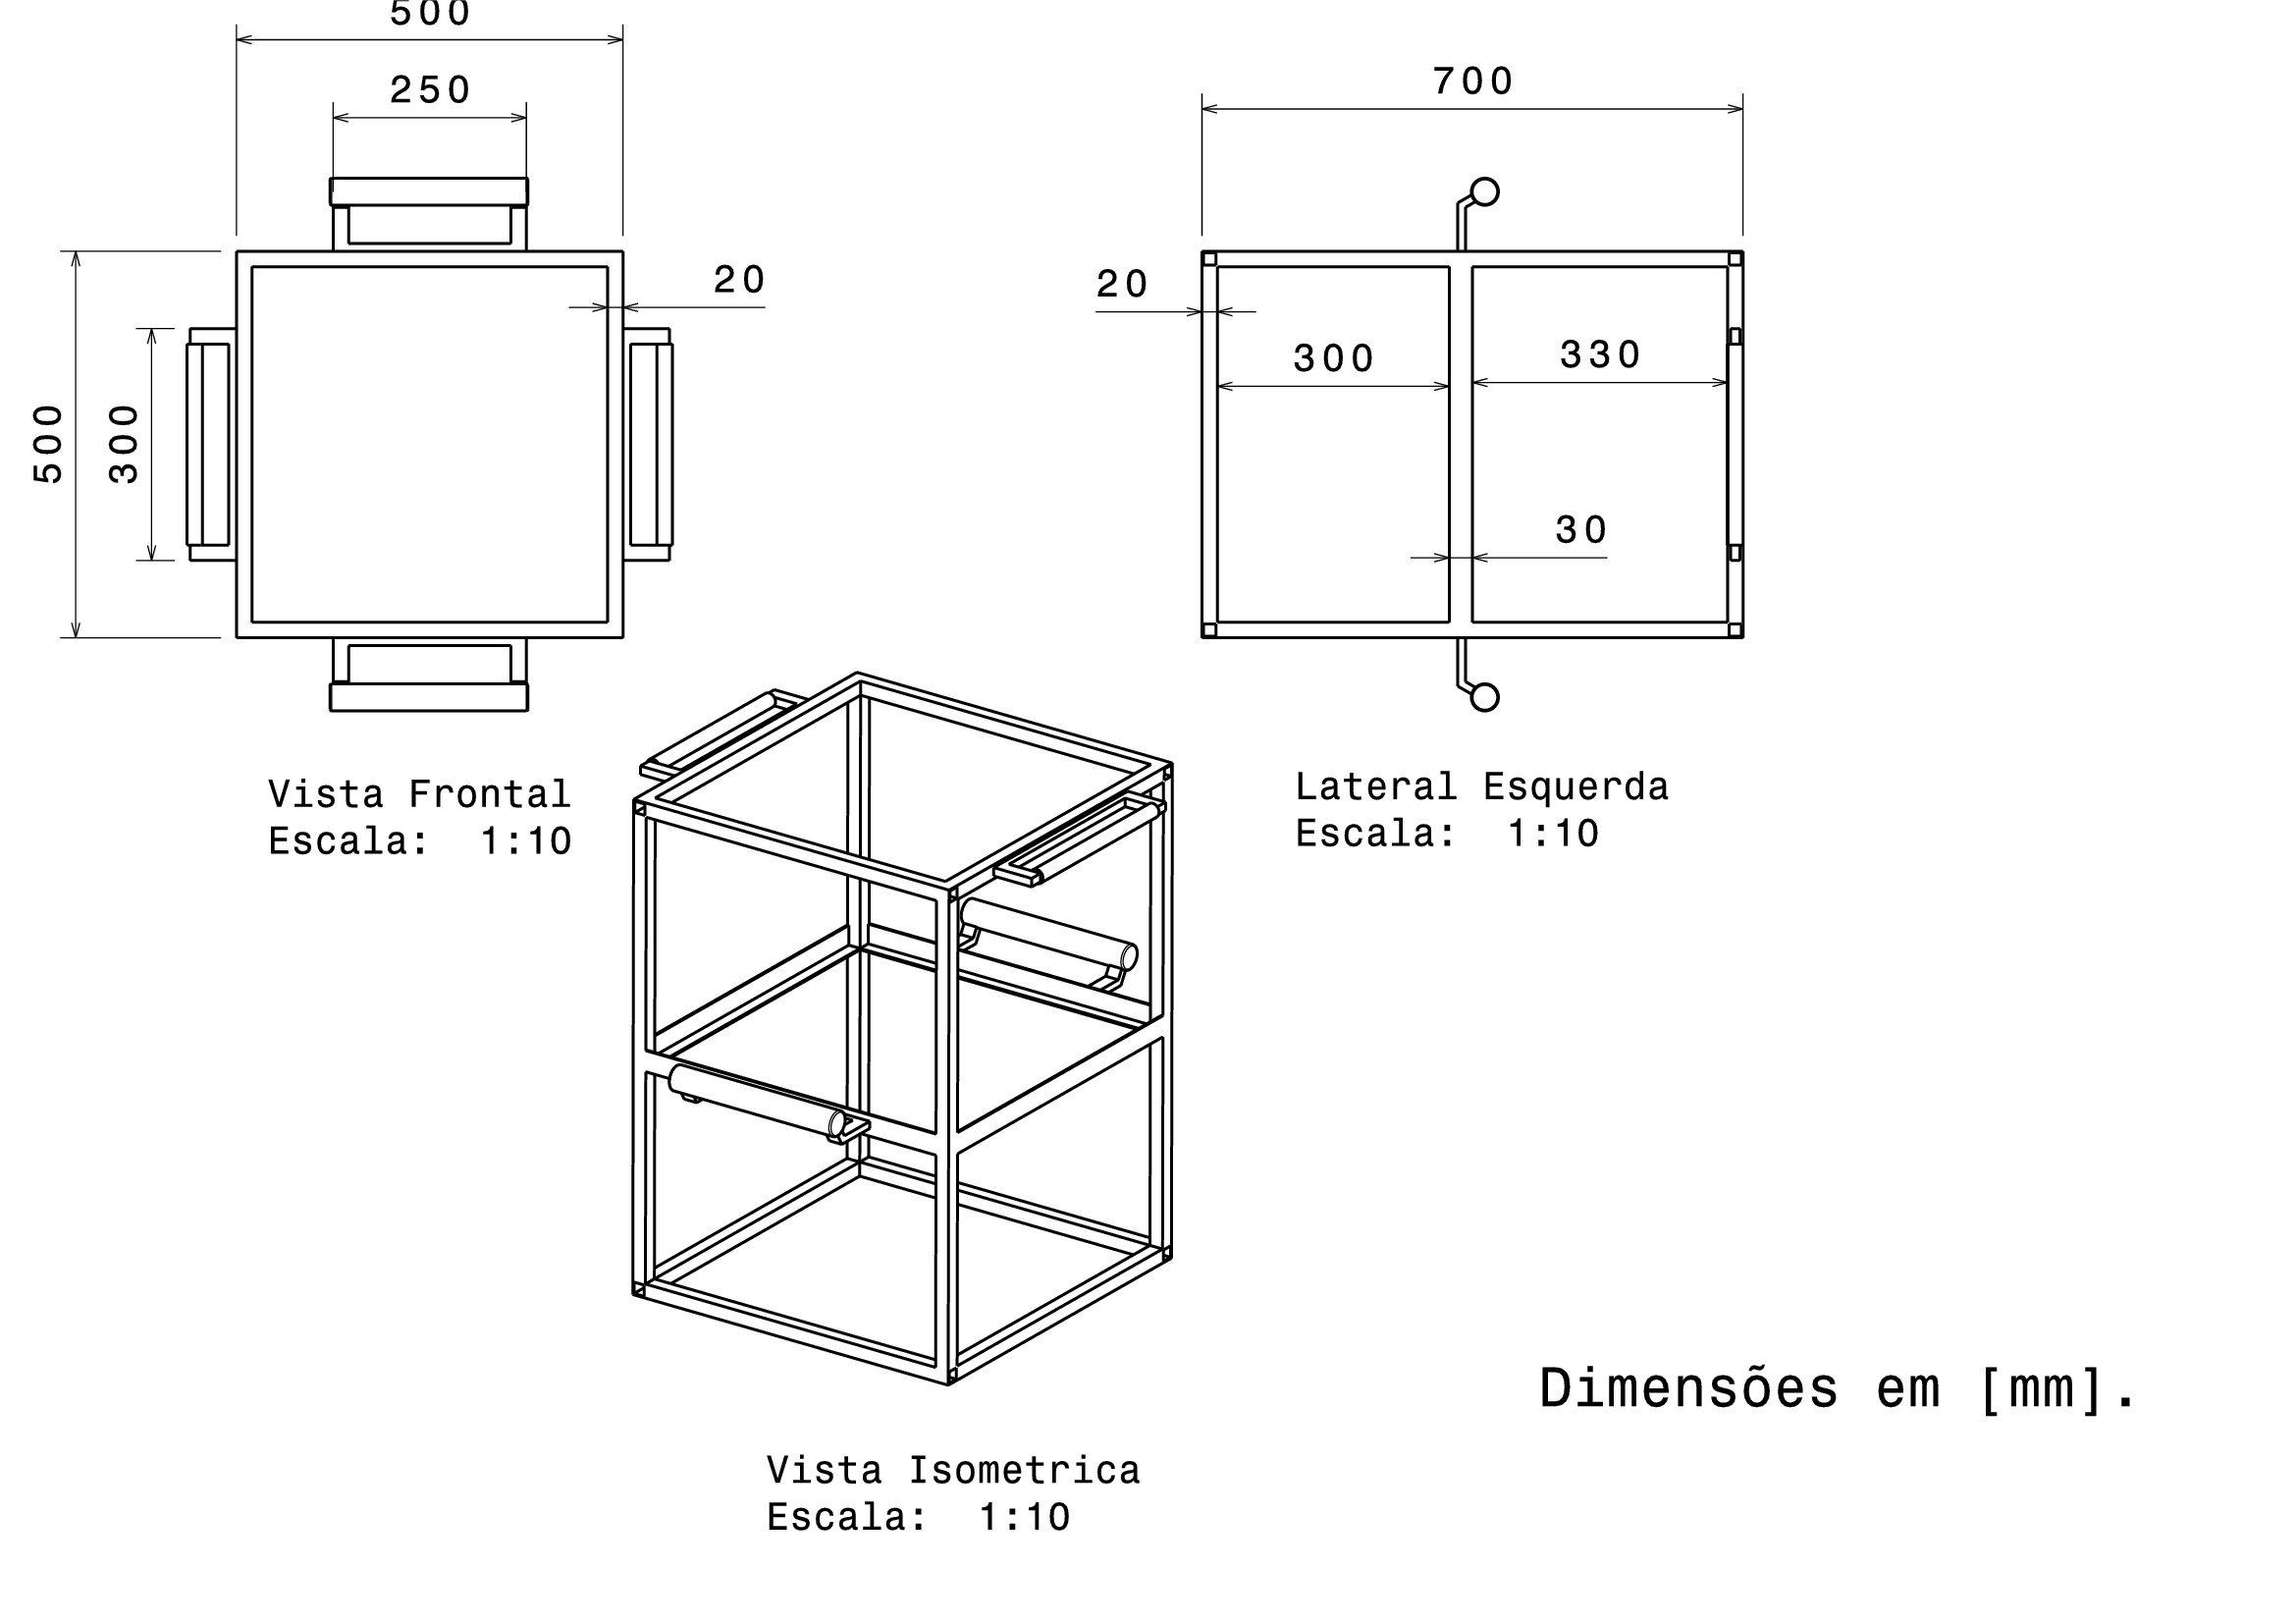
\includegraphics[scale=0.15]{figuras/caixote.png}
\caption{Dimensões da estrutura principal do carrinho}
\end{figure}

\begin{figure}[H]
\centering
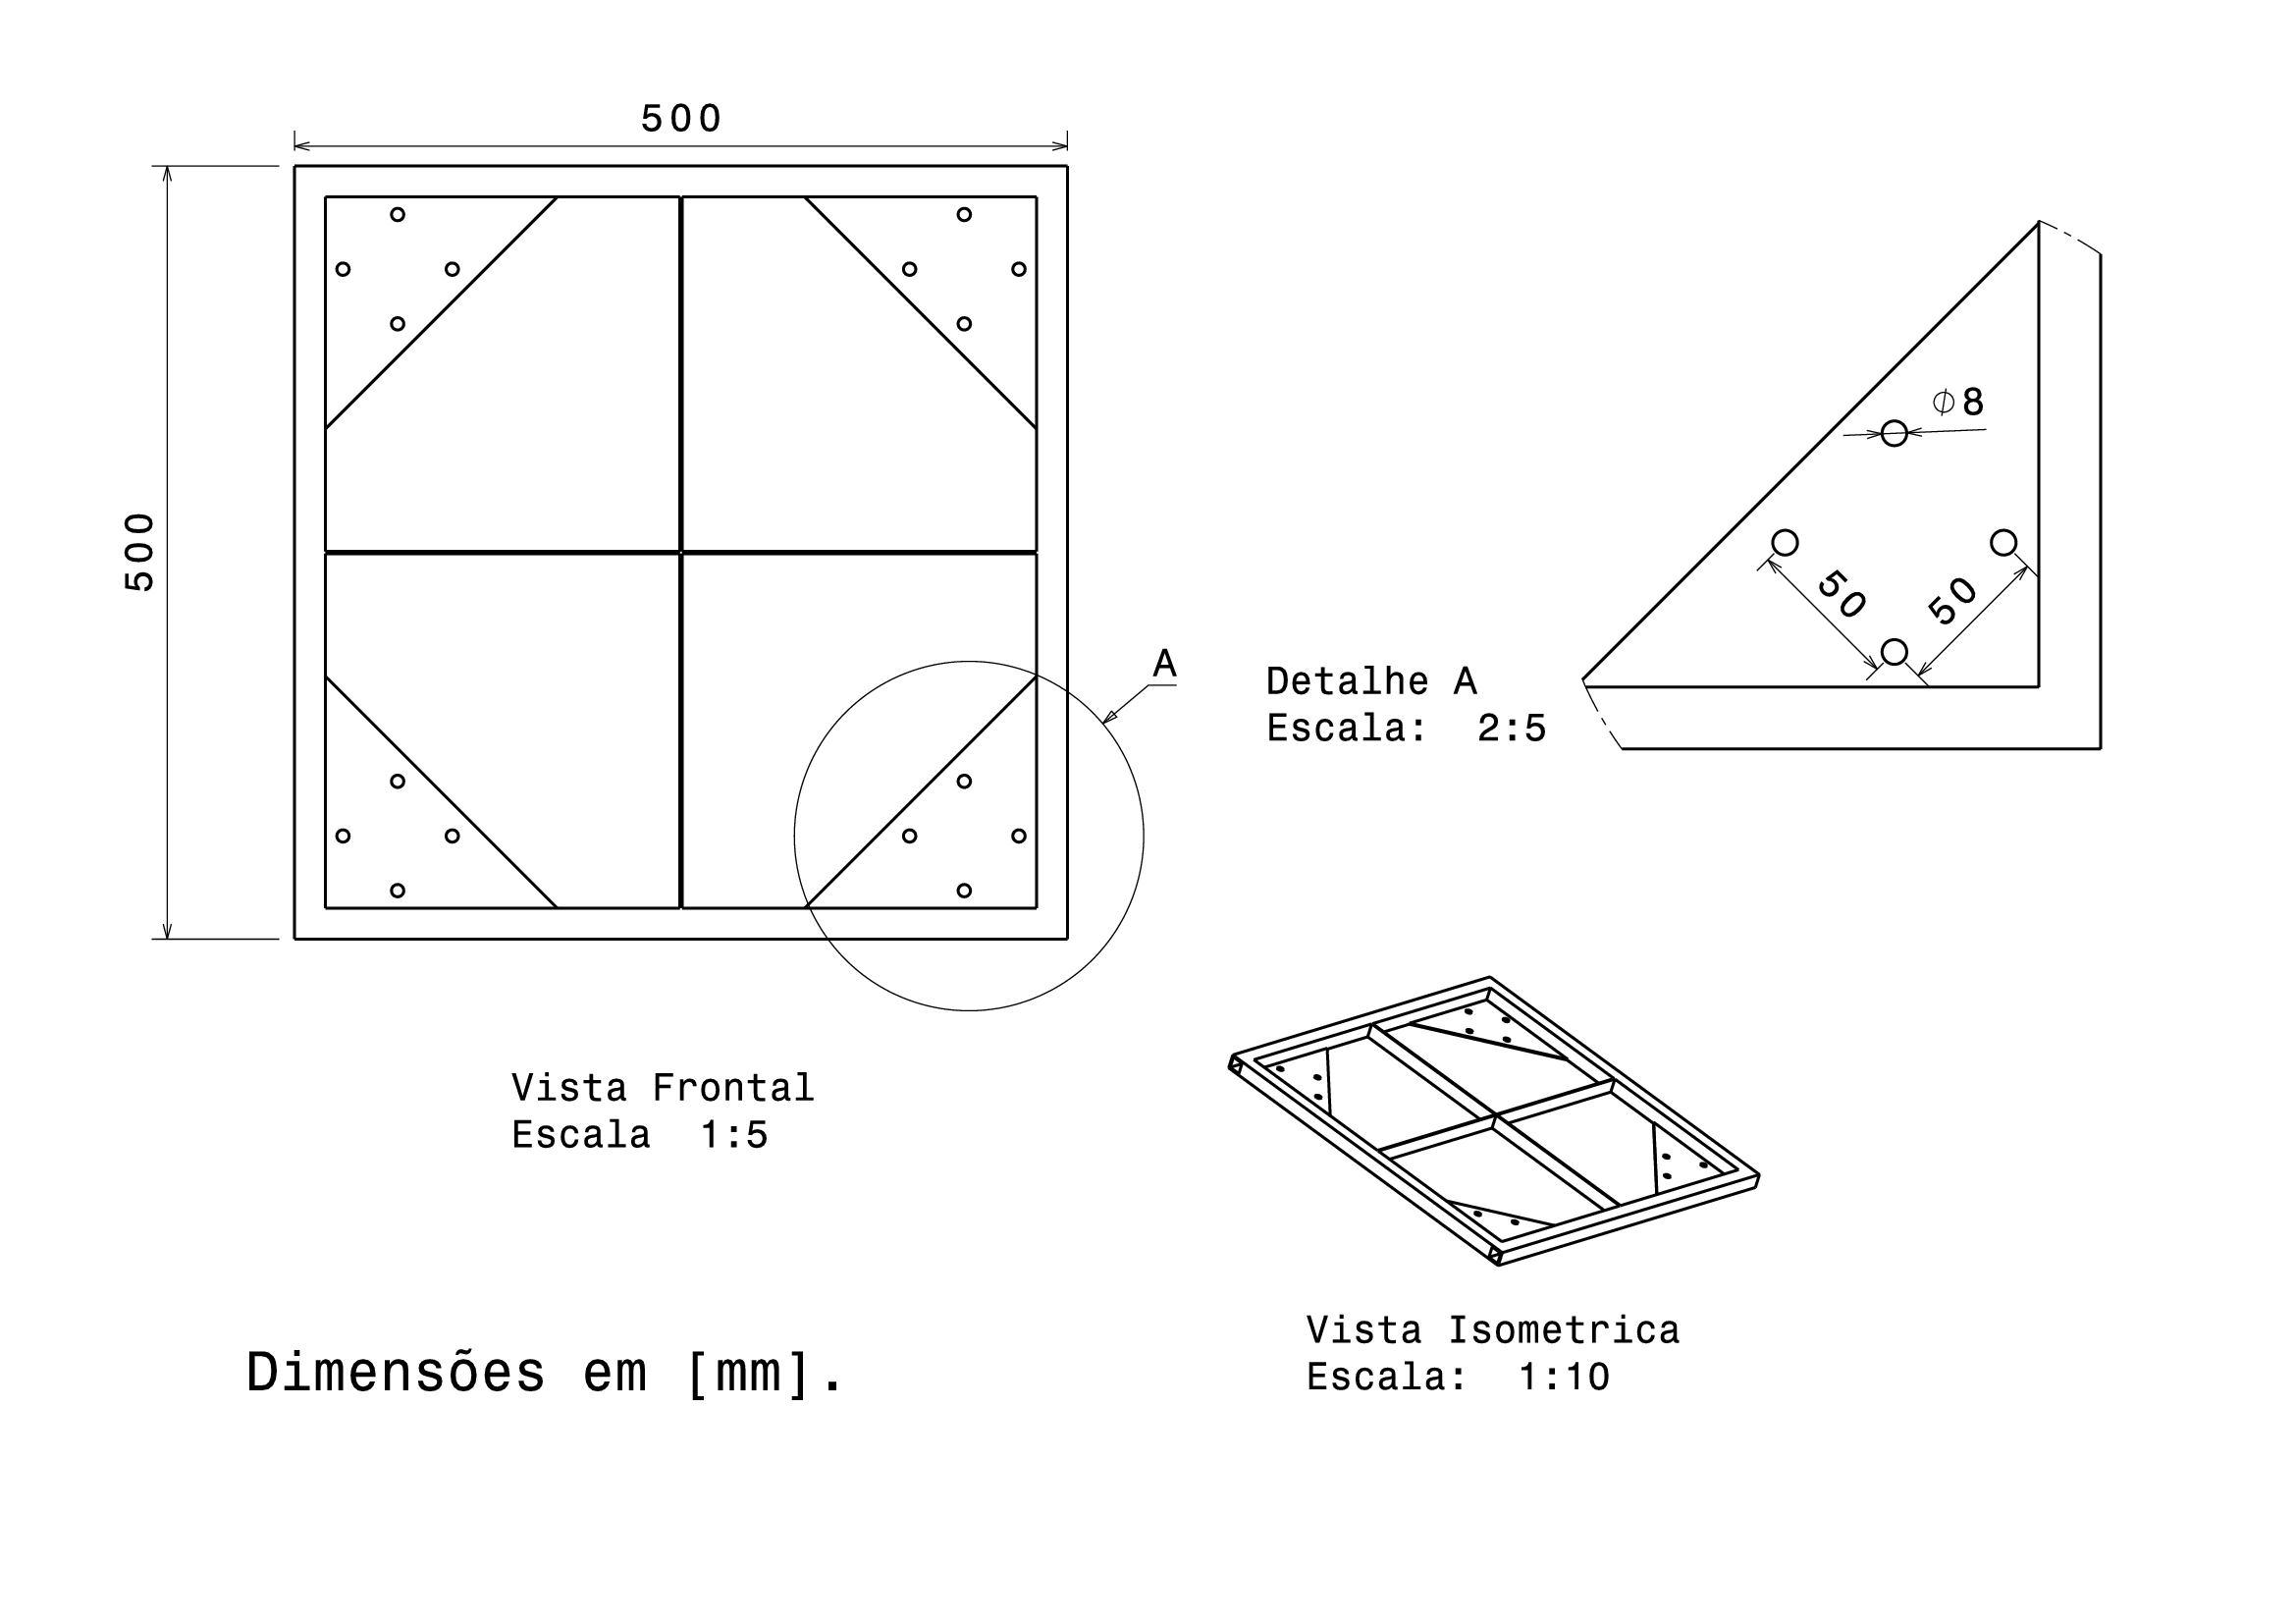
\includegraphics[scale=0.15]{figuras/base.png}
\caption{Dimensões da base de apoio da estrutura}
\end{figure}

\begin{figure}[H]
\centering
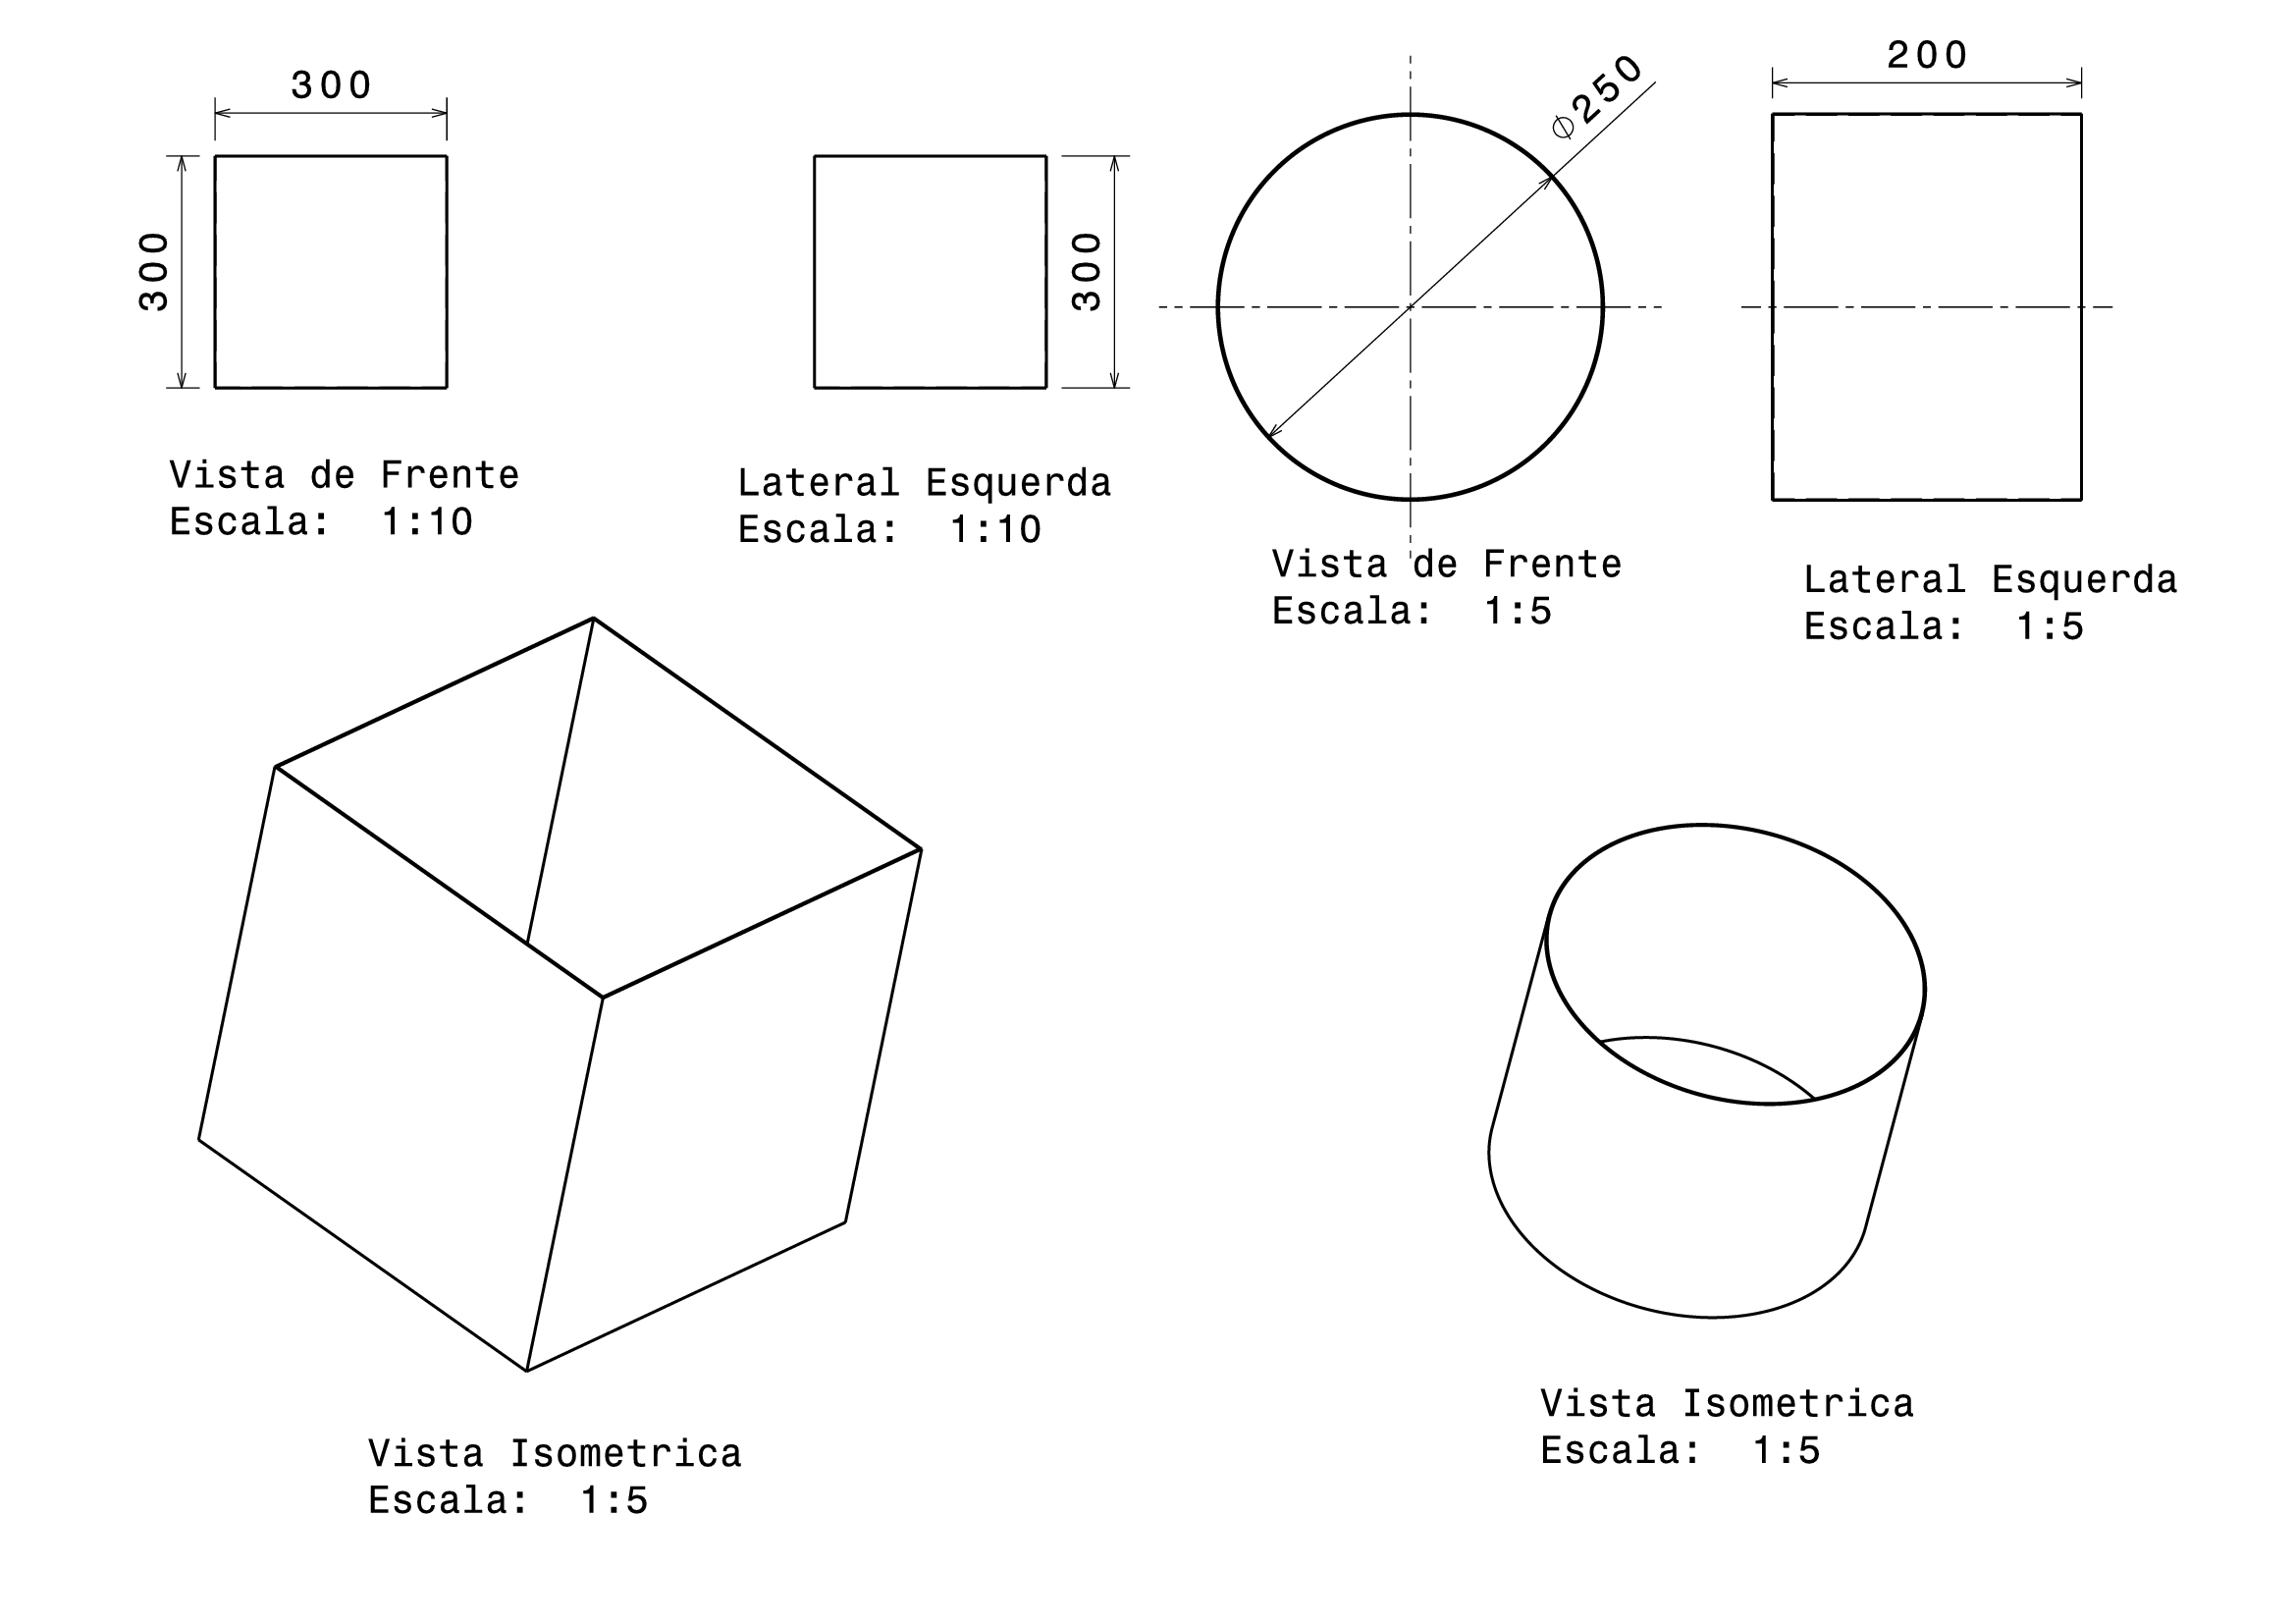
\includegraphics[scale=0.15]{figuras/caixas.png}
\caption{Dimensões dos elementos estruturais internos}
\end{figure}

\subsection{Materiais principais}

O material estrutural tem como objetivo resistir aos esforços durante a utilização da transportadora de órgãos. As cargas de ocorrências durante sua utilização são puramente estáticas, além disso, o projeto deve conciliar baixo custo com baixo peso. Portanto, uma boa opção é o metalon, um aço carbono com costura de baixo custo comumente utilizado em estruturas mecânicas.

\begin{figure}[H]
\centering
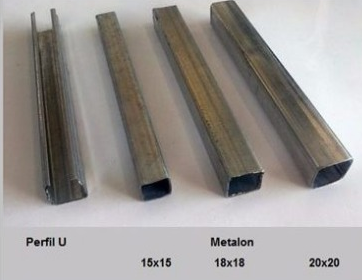
\includegraphics[scale=1]{figuras/metalon.png}
\caption{Perfis de Metalon}
\end{figure}

Para a caixa de alocação de órgãos, foi escolhido o aço inox, devido suas propriedades anticorrosivas e térmicas, aliadas ao baixo custo e maior facilidade de aquisição quando comparado com o aço cirúrgico.

\begin{figure}[H]
\centering

\includegraphics[scale=0.8]{figuras/chapainox.png}
\caption{Chapa de Aço Inox 304}
\end{figure}

A carenagem em volta da estrutura será feita de Policloreto de Vinila (PVC), por ser um material leve e de fácil maneabilidade.

\begin{figure}[H]
\centering

\includegraphics[scale=0.8]{figuras/pvc.png}
\caption{Chapas de Policloreto de Vinila}
\end{figure}

\subsection{Requisitos}

\subsubsection{Requisitos Funcionais}
\begin{itemize}
\item Ser capaz de armazenar o órgão hermeticamente
\item Comportar todos os outros subsistemas
\item Ser móvel e carregável
\item Todas as partes internas do compartimento de carga devem ser capazes de passar por processo de esterilização
\end{itemize}

\subsubsection{Requisitos não-funcionais}

\begin{itemize}
\item Possuir compartimento que possa ser completamente vedado
\item Possuir sistema de rodas para movimentação em solo e alças para carregamento manual
\item Pesar um máximo de 40 kg
\item As peças que serão refrigeradas devem ser resistentes a corrosão
\item Os elementos responsáveis por suportar cargas devem ter resistência para isto
\item O sistema de rodas deve ser capaz de fácil anexagem e desanexagem
\item O compartimento de carga de órgãos deve ser facilmente anexado e desanexado em seu local
\end{itemize}

\subsection{Desafios Técnicos}

\subsubsection{Isolamento térmico da câmara}
Para ajudar a manter uma baixa temperatura estável na câmara fria, é necessário que haja um isolamento térmico em volta do compartimento resfriado. Para isto será feito um revestimento de poliestireno expandido (isopor) ou espuma de poliuretano ao redor da câmara fria.

\subsubsection{Esterilização do sistema}
De acordo com as normas o compartimento no qual o órgão estará contido deve ser esterilizado, portanto deve ser capaz de fácil montagem e desmontagem, o cria um desafio para a fabricação de um compartimento que seja facilmente retirado quando necessário, mas ao mesmo tempo deve estar fixo durante todo o transporte do órgão. Em vista disso, o compartimento estará anexado a estrutura através de peças centralizadoras de seção quadrada com as dimensões da câmara fria e um furo cujo diâmetro é o mesmo do compartimento de carga.
         
\subsubsection{Mobilidade do sistema}
A transportadora possui fácil mobilidade como requisito, o que traz como desafio técnico como será feito o sistema de mobilização de modo estável. A solução que será adotada consiste em módulo que pode ser anexado e desanexado da estrutura principal. Deste modo, quando necessário colocar a transportadora em cima de uma bancada ou algo semelhante, é possível desanexar o módulo de mobilização. O módulo possuirá rodas de baixa vibração e boa capacidade de carga com travas.
\section{Sistemas Eletrônicos}
Com vistas à concepção e validação da solução, foram definidos os requisitos relativos ao subsistema de alimentação e refrigeração do produto:

\subsection{Servidor}
O servidor será construído com auxílio do Rasberry Pi,que é um computador que praticamente o tamanho de um cartão de crédito. Ele foi desenvolvido primeiramente com o intuito de se aprender programação.
Pode ser usado como um substituto para grandes computadores, pois ele permite a
instalação de um sistema operacional, baseado em Linux, como o Raspbian. Com a sua
boa capacidade de processamento ele permite inclusive que se possa jogar certos jogos e
ver vídeos em alta definição. Os pinos de propósito geral de entrada/saída (GPIO,
general purpose input/output) permitem que ela seja usada pra uma grande variedade de
várias aplicações. Esses pinos são pinos de entrada e saída digitais.
 \begin{figure}[H]
 	\begin{center}
 		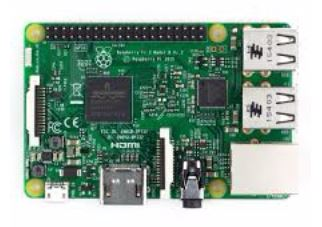
\includegraphics[scale = 0.75]{figuras/Rasp.JPG}
 		\caption{Vista superior da Raspberry}
 	\end{center}
 \end{figure}
A Raspberry Pi 3 possui um processador quad core de 1.2GHz, 64 bits, uma
placa de rede wireles, módulo Bluetooth, 4 portas USB, 40 pinos de entrada e saídas digitais, GPIOs, porta HDMI, por Ethernet, conector de áudio 3.5mm, P2, um slot para cartão micro SD.
Para a sua alimentação, é necessário uma fonte de 5V e de 2A, totalizando um
gasto de energia de 10W. Se a fonte não consegue fornecer uma tensão e essa corrente especificada, a placa de desenvolvimento pode funcionar de uma maneira inadequada e não conseguindo tomar todas as ações necessárias comprometendo o funcionamento do sistema que depende dela como um todo.

A sua utilização, será feita conjunto com outros microcontroladores, pois mesmo
havendo uma alta capacidade de processamento, ela não é muito adequada para
situações em que se necessite processamento quase em tempo real. Isso ocorre pois ela
está em amplo funcionamento com um sistema operacional, o que consome muitos
recursos do processamento.

Para a sua utilização em conjunto, será necessária o uso de um protocolo de
comunicações, como o I2C, SPI ou UART, essa escolha será feita para que se tenha um
melhor aproveitamento da velocidade de comunicação. I2C e SPI, levam uma
vantagem, pois ela permite que seja feito uma rede de comunicação com vários
dispositivos. Isso é permitido, pois se pode haver um mestre, que determina a
velocidade de transmissão, e vários escravos que vão se comunicando com o mestre.
\subsection{Circuito Preventivo}
O circuito preventivo visa proteger o sistema como um todo da ocorrência de sobretensão, evitando assim que se danifique o produto. Ele é feito tendo como base um relé e um diodo Zener. Sua função é interromper a passagem de corrente no momento em que a tensão de entrada ultrapassa um valor limiar. O circuito está ilustrado logo abaixo:
 \begin{figure}[H]
 	\begin{center}
 		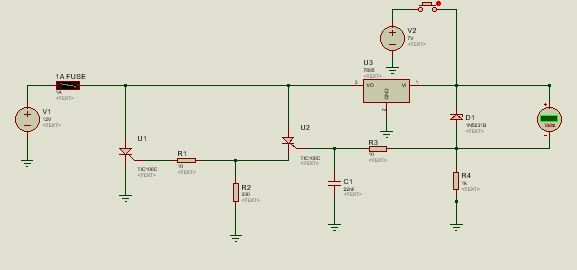
\includegraphics[scale = 0.75]{figuras/Protecao.JPG}
 		\caption{Circuito de proteção}
 	\end{center}
 \end{figure}

\subsection{Controle PWM}
 O controle PWM --- tanto o que agirá sobre o cooler quanto o que agirá sobre a célula peltier --- está ilustrado na figura logo abaixo:
 \begin{figure}[H]
 	\begin{center}
 		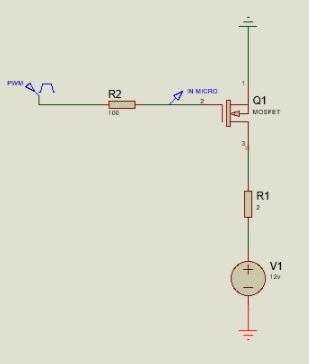
\includegraphics[scale = 0.65]{figuras/Controle_PWM.JPG}
 		\caption{Circuito responsável pelo controle PWN}
 	\end{center}
 \end{figure}
 
	 Ligado a esse circuito, está o controlador MSP430, responsável por utilizar um dos seus pinos como saída PWM para que o circuito acima o amplifique com auxílio do MOSFET. Conforme o datasheet, o pino PWM do MSP430 é o P1.6
\subsubsection{Subsistema de Controle}
O sistema de controle deve ser capaz de:
\begin{itemize}
	\item Realizar a aquisição de dados através de sensores;
	\item Realizar o controle de potência fornecida para os coolers e placa peltier;
	\item Transmitir os dados dados recebidos para outra placa;
	\item Tomada de decisão de acordo com os dados.
\end{itemize}

\subsubsection{Subsistema de Proteção}
O sistema de proteção deve ser capaz de:
\begin{itemize}
	\item Proteger o circuito de sobretensão;
	\item Proteger o circuito de sobrecorrente.
\end{itemize}

\subsubsection{Subsistema de Comunicação e Análise}
O sistema de proteção deve ser capaz de:
\begin{itemize}
	\item Analisar todos os dados advindos de sensores e outros componentes;
	\item Transmitir dados para um servidor WEB;
	\item Transmitir dados usando algum tipo de rede sem fio.	
\end{itemize}


\section{Tabela de custos}

 \begin{figure}[H]
 	\begin{center}
 		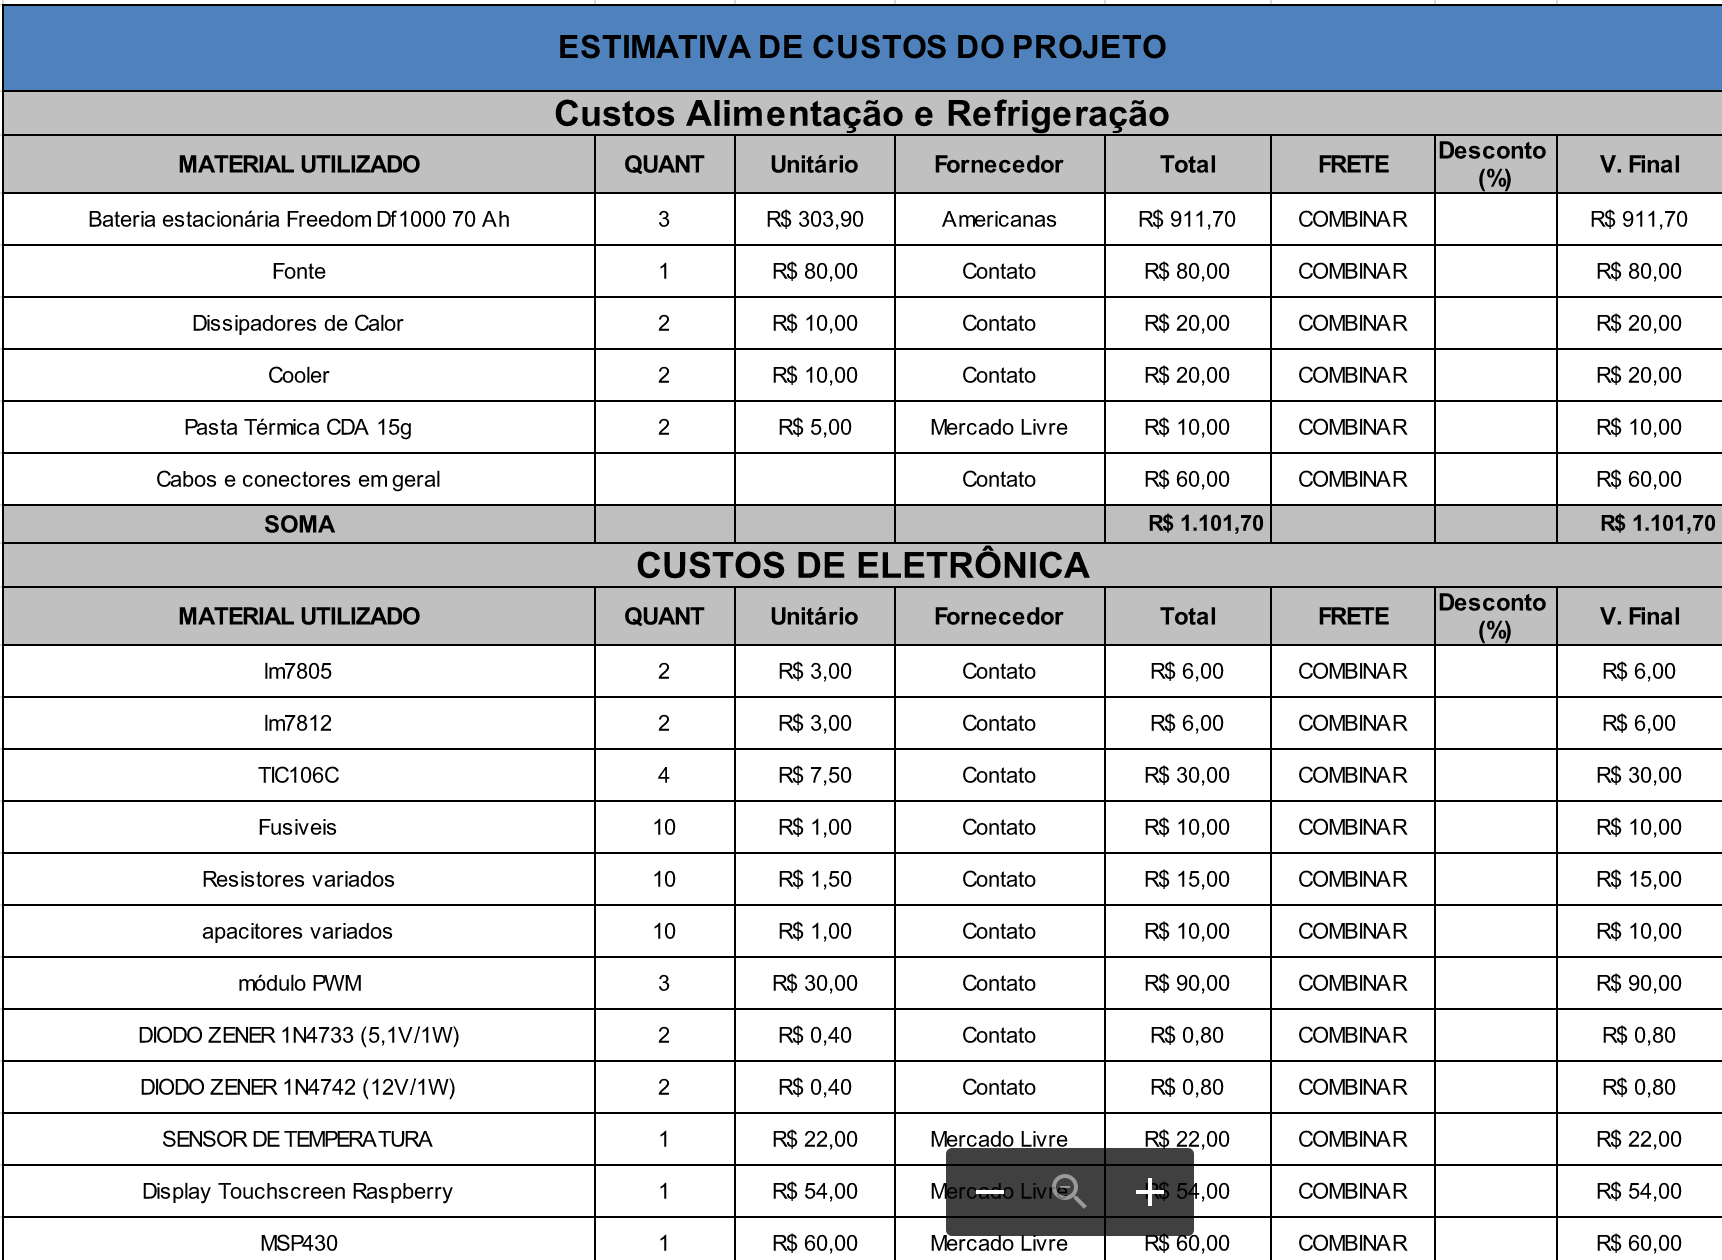
\includegraphics[width=15cm]{figuras/custos.png}
 	\end{center}
 \end{figure}
 
 \begin{figure}[H]
 	\begin{center}
 		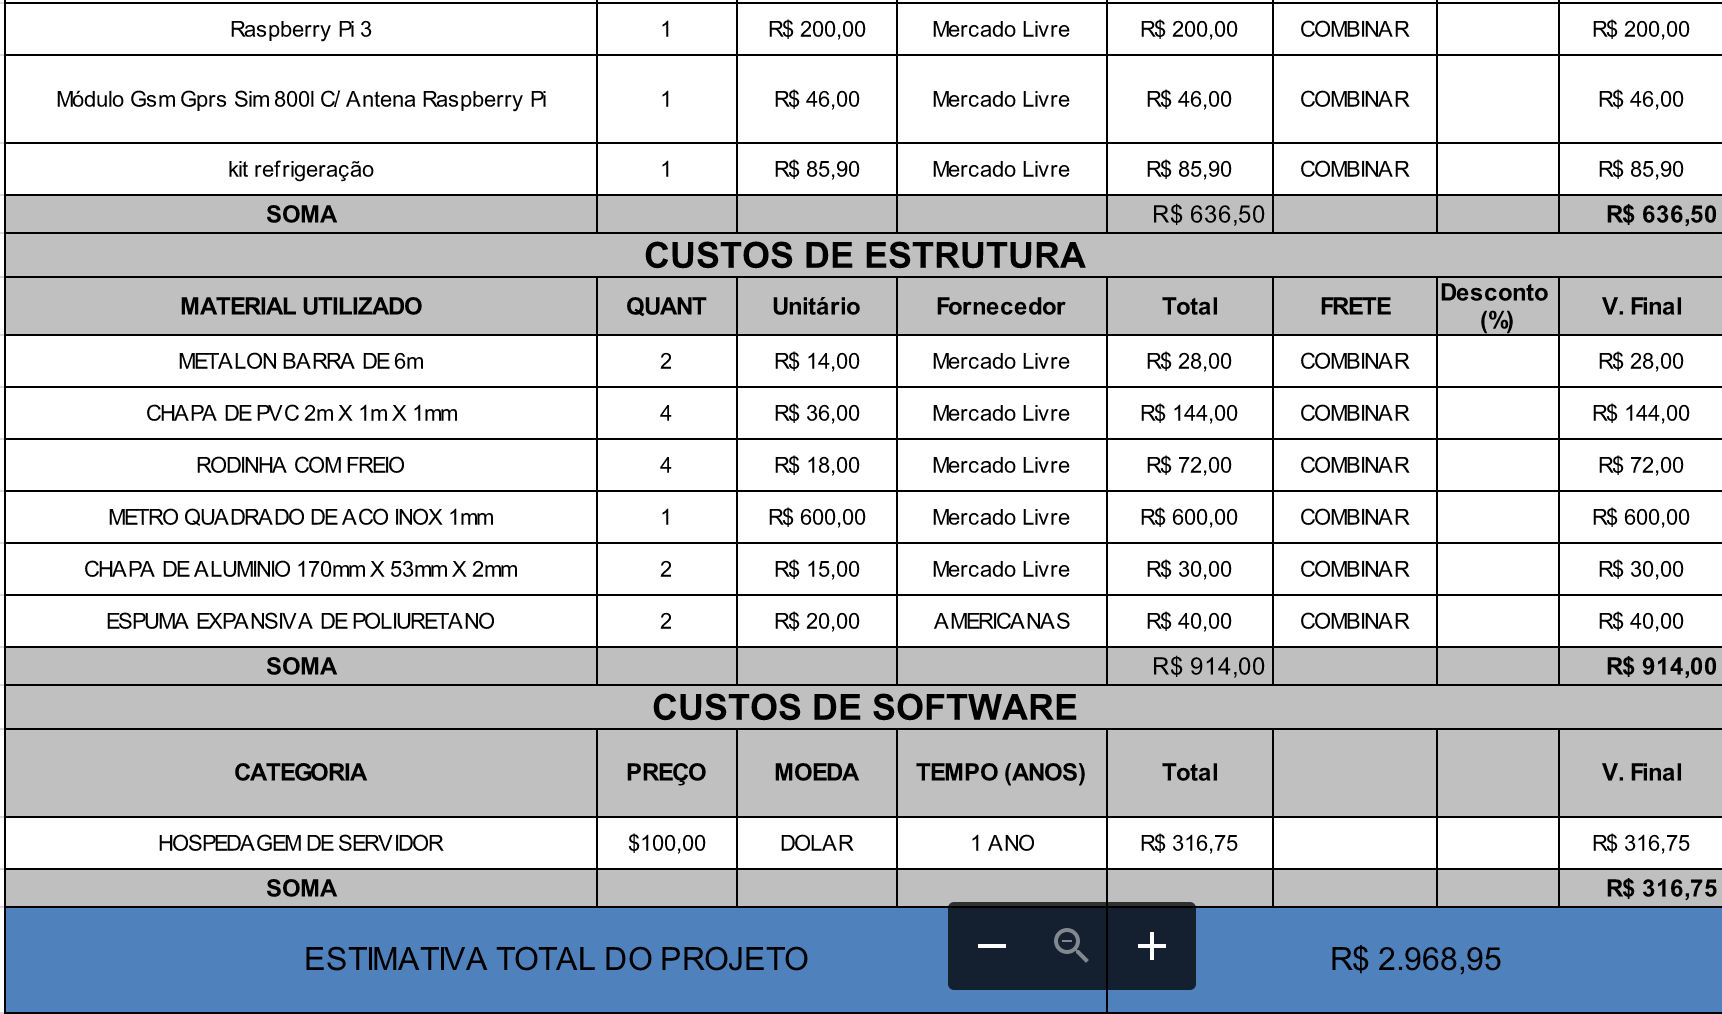
\includegraphics[width = 15cm]{figuras/custos_2.png}
 		\caption{Tabela de custos}
 	\end{center}
 \end{figure}
